%!TEX root =../cmbs4_scibook.tex
%%%%%% CMB-S4 DE/DM Chapter  %%%%%%%%%%%%%%%%

\chapter{Dark Energy}

\section{Dark Energy and Modified Gravity}

\begin{center}
{\small \it (send feedback on this chapter to \href{mailto:s4_de@cosmo.uchicago.edu}{s4\_de@cosmo.uchicago.edu})}
\end{center}

The enigma of cosmic acceleration is among the most challenging problems in physics. Our most basic understanding about gravity -- that objects fall towards one and other under mutual gravitational attraction -- simply does not apply on the largest distance scales. Instead, gravity is apparently repulsive at large distances and late times; the scale of spacetime itself is currently not only expanding but accelerating. The implication is either that our understanding of gravity is incomplete, or some other causative agent -- dark energy -- with exotic gravitational properties fills the universe. In both cases, new physics is required beyond the four fundamental forces described by the Standard Model and general relativity.

The working hypothesis is that the cosmic acceleration is due to an exquisitely small cosmological constant, that Einstein's general relativity is valid from millimeter to beyond gigaparsec scales, and that dark matter consists of a single species of a cold, collisionless particle. Yet none of these offer insight or reflect the unity of physics demonstrated elsewhere as in the Standard Model of particle physics.

In particular, the cosmological constant suffers from a naturalness problem whose resolution may lie in a dynamical dark energy, quintessence. Theories of quintessence posit a new scalar field and predict a variety of testable phenomena.  They can also unveil new links to dark matter, neutrino physics, and cosmic parity violation. In their most general form, they represent
a scalar-tensor theory of gravity which can be described by  the effective field theory (EFT) of cosmic acceleration in the linear regime. 
CMB-S4 can provide the hard evidence  needed to pare down these possibilities and potentially discover clues to the enigma of cosmic acceleration that will enable the development of  compelling theoretical 
alternatives to the cosmological constant.

% possibly redundant... eventually streamline.
In summary, the current observational evidence suggests a new frontier for physics at low energies and weak coupling, implied by the cosmological scales that characterize cosmic acceleration.CMB lensing, thermal SZ cluster counts and mass measurements, and the kinematic SZ effect  all measure the influence of cosmic acceleration on the growth of 
structure.   As such, CMB-S4 would be capable of helping to answer basic questions about dark energy and gravity in a manner complementary to ongoing precision measurements of the expansion history.    % and dark matter (restore later if we merge).


\subsection{Models and parameters}
In this section, we  briefly review the models and frameworks that have been proposed over the past years to test dark energy and modified gravity.   These fall into 
three families: ``trigger'', equations of motion, and theory parametrizations. The first ones are aimed at testing and falsifying the standard model
of $\Lambda$CDM, a cosmological constant with cold dark matter, and are agnostic as to its 
alternatives.  Given precise measurements from primary CMB anisotropy of the high redshift universe, all low redshift observables related to the expansion history and growth of
structure are potential triggers.  Trigger parameters thus have the benefit that their relationship to the raw observables can be made as direct as desired.   The drawback is 
that deviant values for the trigger may not have any physical motivation.  Instead they help pare down the possibilities for the more model
dependent and theory oriented tests.  


  In the next section we discuss the cluster abundance,
 CMB lensing and pairwise kinematic SZ effects as the building blocks of triggers when
 combined with other measurements such as BAO and SNIa.   CMB-S4 will also enhance the precision and robustness
 of these other tests by measurements of the primary $E$-mode polarization.   For example
 the cold dark matter $\Omega_c h^2$ and effective relativistic degrees of freedom $N_{\rm eff}$ enter into the calibration of the BAO scale as well as inferences on $H_0$. 
 
In addition to triggers based on the expansion history, CMB-S4 provides triggers based
on the growth of structure.  The $\Lambda$CDM model predicts that the growth of structure
will slow in a precisely known manner as the expansion starts to accelerate.   
For example the rms amplitude of linear matter fluctuations at the $8 h^{-1}$Mpc
scale $\sigma_8(z)$ is a trigger parameter that can be closely associated with the 
cluster abundance.   The linear growth rate index $\gamma$ is another that is closely related
to peculiar velocities and the kSZ observables.   
% add in $E_G$ if we forecast it or if it is discussed in the cross correlation section.

The second way of parametrizing deviations from $\Lambda$CDM is by modifying the equations of motion for dark energy in a manner consistent with conservation laws.   These have the benefit of attempting to tie distance and growth
tests together in a physical, yet still phenomenological manner.    The next step up in
complexity from a cosmological constant is a model where the dark energy is dynamical
but spatially smooth relative to the dark matter.   In these models, the expansion history
can deviate from that of $\Lambda$CDM due to evolution in  the dark energy
equation of state $w(z)$, yet still predict the growth of structure.   A common parameterization
of this phenomenology is
\begin{equation}
w(z) = w_0 + w_a \frac{z}{1+z}.
\end{equation}
The figure of merit defined by the DETF is the inverse area of the
95\% CL region in the $w_0-w_a$ plane.  

There are generalizations of this type of parameterization that separate the expansion history from 
the growth of structure.   
A complete parametrization for observables for scalar-tensor theories in the linear regime would include in addition
the gravitational slip or effective anisotropic stress  (the ratio of the space curvature potential and Newtonian potential),  the effective Newton constant, and  $c_T$ the
speed of tensor perturbations. [intentionally vague on which notation to use: forecaster will
decide the favorite one and supply details.  Possibly add graviton mass as it is mentioned
in Inflation chapter.]

%
The last way of studying deviations from $\Lambda$CDM consists in directly testing theories beyond it.  Given the lack of a compelling specific theory to test, we can still make progress
by parameterizing all possible Lagrangians for fluctuations that are consistent with the
given symmetry.
 This approach maintains a strong connection with the underlying theory at the price of
complicating the relation to the raw data.  

More specifically, a systematic implementation of this approach is the effective field theory (EFT)
of cosmic acceleration \cite{Gubitosi:2012hu,Bloomfield:2012ff}, inspired by the EFT  of inflation described in the Inflation Chapter~\cite{Creminelli:2006xe,Cheung:2007st,Weinberg:2008hq,Creminelli:2008wc,Park:2010cw,Jimenez:2011nn}.    The EFT of cosmic acceleration describes the cosmological phenomenology of all universally coupled single scalar field dark energy and modified gravity models. Specifically, the EFT action is constructed in a unitary gauge to preserve isotropy and homogeneity of the cosmological background and reads:
%
\begin{eqnarray} \label{Eq:EFTaction}
\mathcal{S}_{\rm EFT} = \int d^4x \sqrt{-g}&& \bigg\{ \frac{m_0^2}{2} \left[1+\Omega(\tau)\right] R + \Lambda(\tau) - c(\tau)\,a^2\delta g^{00} + \frac{M_2^4 (\tau)}{2} \left( a^2\delta g^{00} \right)^2 \nonumber \\ 
&&   - \frac{\bar{M}_1^3 (\tau)}{2} \, a^2\delta g^{00}\,\delta K{^\mu_{\,\,\mu}}  - \frac{\bar{M}_2^2 (\tau)}{2} \left( \delta {K}{^\mu_{\,\,\mu}}\right)^2   - \frac{\bar{M}_3^2 (\tau)}{2} \,\delta {K}{^\mu_{\,\,\nu}}\,\delta {K}{^\nu_{\,\,\mu}} \nonumber \\
&& + m_2^2(\tau)\left(g^{\mu\nu}+n^{\mu} n^{\nu}\right)\partial_{\mu}(a^2g^{00})\partial_{\nu}(a^2g^{00}) +\frac{\hat{M}^2(\tau)}{2} \, a^2 \delta g^{00}\,\delta \mathcal{R}+	\ldots \bigg\}  \nonumber \\
&& + S_{m} [g_{\mu \nu}, \chi_m ]
\end{eqnarray}
%
where $R$ is the four-dimensional Ricci scalar, $\delta g^{00}$, $\delta K{^\mu_{\,\,\nu}}$, $\delta K{^\mu_{\,\,\mu}}$ and  $\delta \mathcal{R}$ are, respectively, the perturbations of the upper time-time component of the metric, the extrinsic curvature and its trace and the three dimensional spatial Ricci scalar of constant-time hypersurfaces. Finally,  $S_m$ denotes the action for all the matter fields conventionally considered in cosmology. 

In the action (\ref{Eq:EFTaction}), the  extra scalar degree of freedom is hidden inside metric perturbations. 
To study the dynamics of linear perturbations, however, it is convenient to make it explicit by means of  the St\"{u}ckelberg technique i.e.~performing an infinitesimal coordinate transformation such that $\tau\rightarrow \tau+\pi$, where the field $\pi$ describes the extra propagating degree of freedom. This approach allows us to maintain a direct link to the underlying theory so that we can keep under control its theoretical viability while exploring the cosmological implications of any of the models included in this language~\cite{Raveri:2014cka}. 

Since the choice of the unitary gauge breaks time diffeomorphism invariance, each operator allowed by the residual symmetry, in action (\ref{Eq:EFTaction}), can be multiplied by a time-dependent coefficient that we shall call EFT function. To fully specify the phenomenology of linear perturbations only a restricted set of EFT functions are needed. These can be either parametrized to explore agnostically the space of dark energy and modified gravity models~\cite{Gleyzes:2013ooa,Bloomfield:2013efa,Piazza:2013coa,Gleyzes:2014rba} or can be fixed to reproduce exactly the phenomenology of some model of interest such as $f(R)$ gravity, quintessence and, more generally, the Horndeski class of theories and beyond~\cite{Gleyzes:2014dya,Frusciante:2015maa,Frusciante:2016xoj}.
%

\section{Cosmic Birefringence}
\label{sec-biref}
The simplest dynamical way to model the accelerated expansion of the universe is to invoke a new slowly evolving scalar field that dominates its energy budget (the quintessence models for DE). Such a field generically couples to photons through the Chern-Simons term in the electromagnetic Lagrangian, causing linear polarization of photons propagating cosmological distances to rotate---the effect known as cosmic birefringence~\cite{Carroll:1998zi}. In the case of the CMB, such rotation converts the primordial E mode into B mode, producing characteristic TB and EB cross-correlations in the CMB maps \cite{Kamionkowski:2008fp,Gluscevic:2009mm}. Even though there is no firm theoretical prediction for the size of this effect, if observed, it would be a clear “smoking-gun” evidence for physics beyond the standard model in the form of a new scalar field. Previous studies have used quadratic estimator formalism to constrain this effect \cite{Gluscevic:2012me}, with the best current limit coming from sub-degree scale polarization measurements with POLARBEAR \cite{Ade:2015cao} ($<0.33$ deg$^2$ for the amplitude of a scale-invariant rotation-angle power spectrum). A promising way to pursue search for cosmic birefringence in the future is measurement of the off-diagonal EB cross correlations on small angular scales, and the measurement of polarization anisotropy on a wide range of scales is going to be essential for achieving this. 

Fig.~\ref{fig:CB-forecast} shows the current upper limit on the rotation-angle power spectrum from POLARBEAR and a projection for Planck, and a forecast for a Stage-IV experiment (with noise of $1.41$ $\mu$K-arcmin in polarization, and a resolution of 1'). The improvement from the current constraint at all multipoles is about two orders of magnitude. We assumed access to polarization modes from $\ell=30$ to $\ell=5000$.
\begin{figure}[h!]
\centering 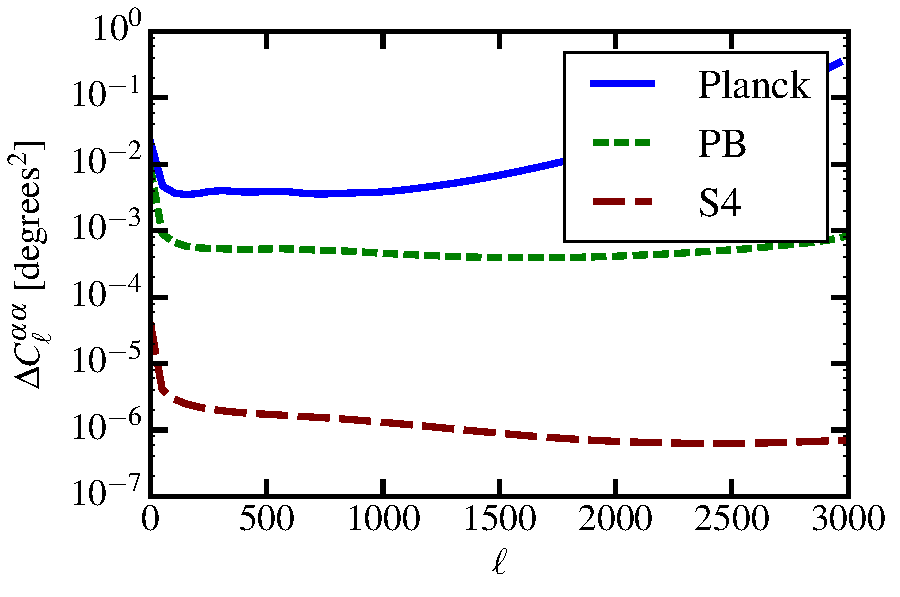
\includegraphics[width=0.70\textwidth]{DarkEnergy/birefringence-S4-planck-PB-v2.pdf}
\caption{The current (from POLARBEAR, labeled as PB) and projected (for Planck and Stage-IV experiment) 1$\sigma$ errobars on the birefringent rotation-angle power spectrum are shown on the vertical axis. A Stage-IV has the potential to improve the current best constraint on anisotropic birefringence by more than two orders of magnitude at all multipoles. For the Stage-IV forecast, we assumed noise of $1.41$ $\mu$K-arcmin (in polarization), a resolution of 1', and have considered polarization modes from $\ell=30$ to $\ell=5000$.}
\label{fig:CB-forecast}
\end{figure}

For a fixed integration time (and a varied noise level and sky coverage), large sky coverage optimizes sensitivity to low multipoles of the rotation angle and gives the best signal-to-noise ratio for rotation models that have power on large scales (such as, for example, a model with a scale-invariant power spectrum, which could result from fluctuations in a spectator scalar field present during inflation). Conversely, for models that have power on scales corresponding to multipoles above $\ell\sim 1000$, best signal-to-noise is achieved with deeper integration on small sky patches.  For a measurement of the magnitude of the quadrupole of the rotation angle, reducing the resolution from 1' to 9' produces a factor of a few increase in the projected errorbar (for all other parameters fixed). Increasing the noise from $1.41$ to $12.7$ $\mu$K-arcmin produces a factor of about $20$ increase in the errorbar. Access to polarization modes down to $\ell=2$ does not significantly affect the forecasts. 

\section{CMB  Dark Energy Observables}

\subsection{Cluster abundance and mass}

Clusters of galaxies are sensitive to the content, geometry, and growth of structure in the universe.     In the report of the DETF, they were highlighted as having the highest sensitivity
to dark energy parameters  but simultaneously the largest astrophysical systematic due
to uncertainties in the mass scaling of the cluster observables.   In the ``Stage IV" era of
dark energy probes, CMB-S4 will play a critical role in overcoming this challenge.




Clusters of galaxies are the most massive ($\sim$10$^{14}$-10$^{15}$ M$_{\odot}$) objects in the universe to have underwent gravitational collapse, 
having formed from regions $\sim$10-40 Mpc.  This property makes clusters representative of the overall content of the universe, and also makes them 
important tracers of the evolution of large-scale structure, sampling the most extreme peaks in the large-scale matter distribution.  
These properties have enabled clusters to make important contributions to cosmology: the discovery of dark matter in the 
Coma cluster \cite{Zwicky:1933gu}, 
providing early evidence for $\Omega_m < 1$ \cite{White:1993wm, Donahue:1997sp, Bahcall:1998ur}, and
constraining the physical nature of dark matter \cite{Clowe:2006eq}.  
More recently, measurements of clusters have been used to constrain the properties of dark energy and modifications 
to gravity \cite{Vikhlinin:2008ym, Mantz:2009fw, Rapetti:2012bu, Benson:2011uta, Mantz:2014xba, Mantz:2014paa}.   In the future era of ``Stage IV'' dark energy 
facilities such as DESI and LSST, measurements of the abundance of galaxy clusters can make complementary and 
competitive constraints on the dark energy equation of state and deviations from General Relativity \cite{Weinberg:2012es}.  

CMB measurements find clusters through the inverse Compton scattering of CMB photons off of intra-cluster gas, otherwise 
known as the Sunyaev-Zel'dovich (SZ) effect \cite{Sunyaev:1972eq}. SZ cluster surveys have two important advantages: 
the SZ surface brightness is redshift independent, and the integrated SZ signal is expected to be a relatively 
low-scatter cluster observable \cite{Nagai:2005wx, Nagai:2007mt, Kravtsov:2012zs}.  These properties enable SZ surveys to provide 
relatively clean, mass-limited cluster catalogs out to high-redshift ($z > 1$).  Since the first SZ-discovered clusters were 
report in 2009 \cite{Staniszewski:2008ma}, SZ surveys have produced catalogs of over 1000 SZ-selected clusters extending out to $z \sim 1.7$ 
\cite{Vanderlinde:2010eb, Reichardt:2012yj, Hasselfield:2013wf, Ade:2013skr, Bleem:2014iim, Ade:2015mva}.  


Figure \ref{fig:limits} shows an estimate of the mass sensitivity, expressed as the one-sigma mass uncertainty as a function of redshift, for two possible CMB-S4 configurations and compares them to planned CMB experiments. 
In Figure \ref{fig:cluster_counts}, we show projections for the mass-threshold and total cluster counts for three possible CMB-S4 configurations.  
The 50\% mass-completeness threshold for the CMB-S4 cluster survey would be relatively flat with redshift out to $z \sim 2$.  
The mass-threshold increases from $\sim$1-2 $\times$ 10$^{14}$ M$_{\odot}$, going from a CMB-S4 angular resolution 
of 1 to 3 arc-minutes, which is $>$2 times lower than current SZ surveys even in the worse case scenario for CMB-S4.  
In addition, the lower mass threshold and larger sky area of CMB-S4, would translate to a nearly $\sim$100 fold increase in the 
number of SZ-identified clusters.  At a 99\% purity threshold, for a configuration with a 1, 2, and arc-minute angular 
resolution, CMB-S4 would identify $\sim$40,000, 70,000, and 140,000 clusters, respectively.  


\begin{figure}[t]
\begin{center}
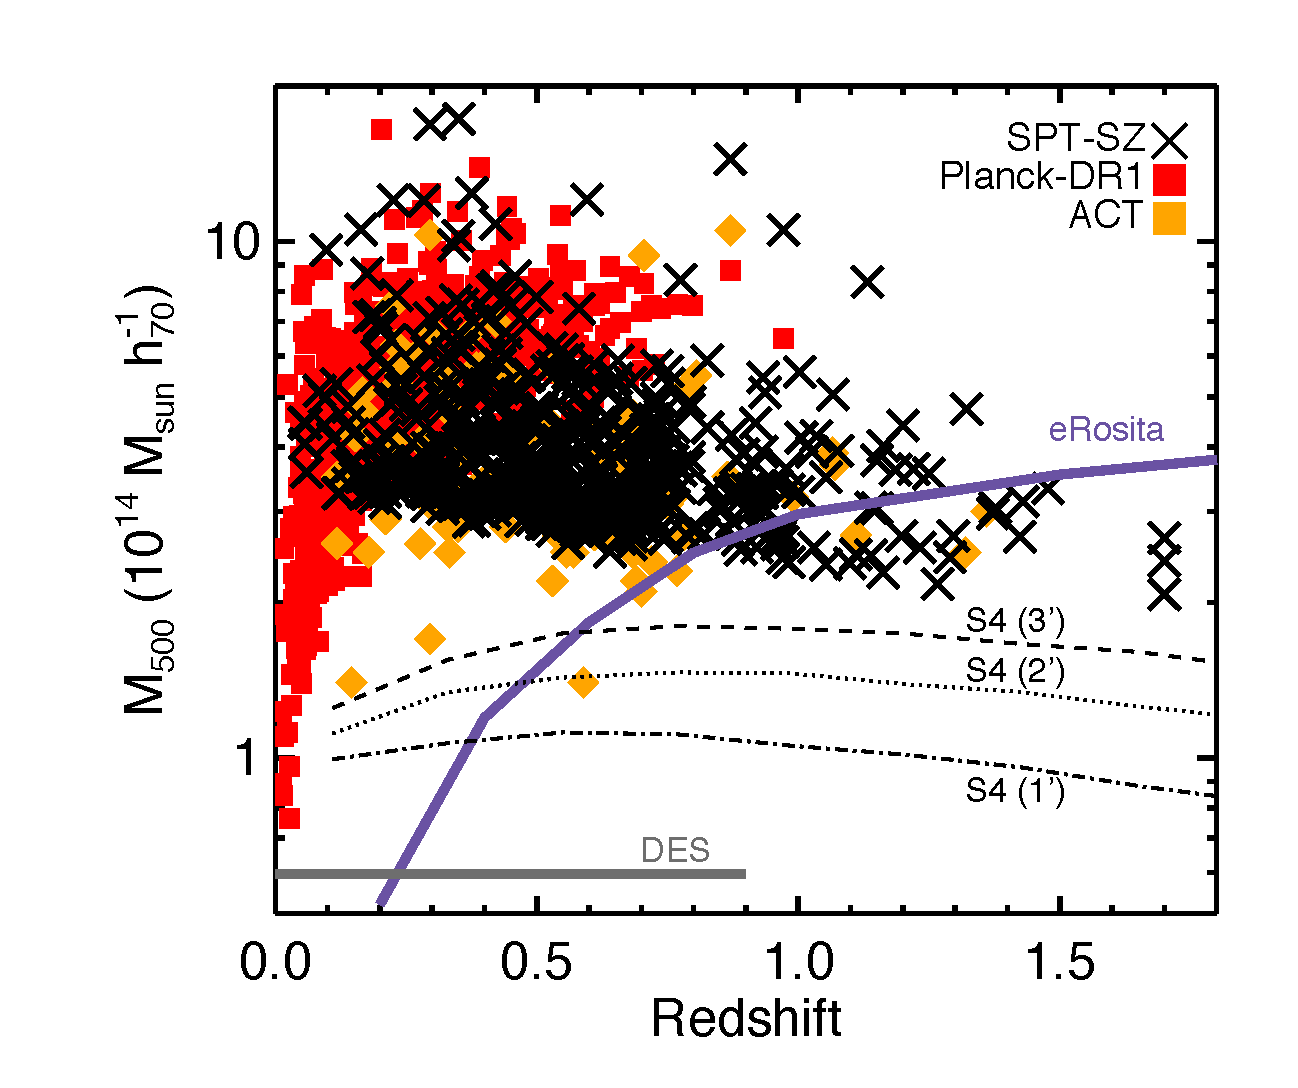
\includegraphics[width=0.49\textwidth]{DarkEnergy/mass_vs_z_s4.pdf}
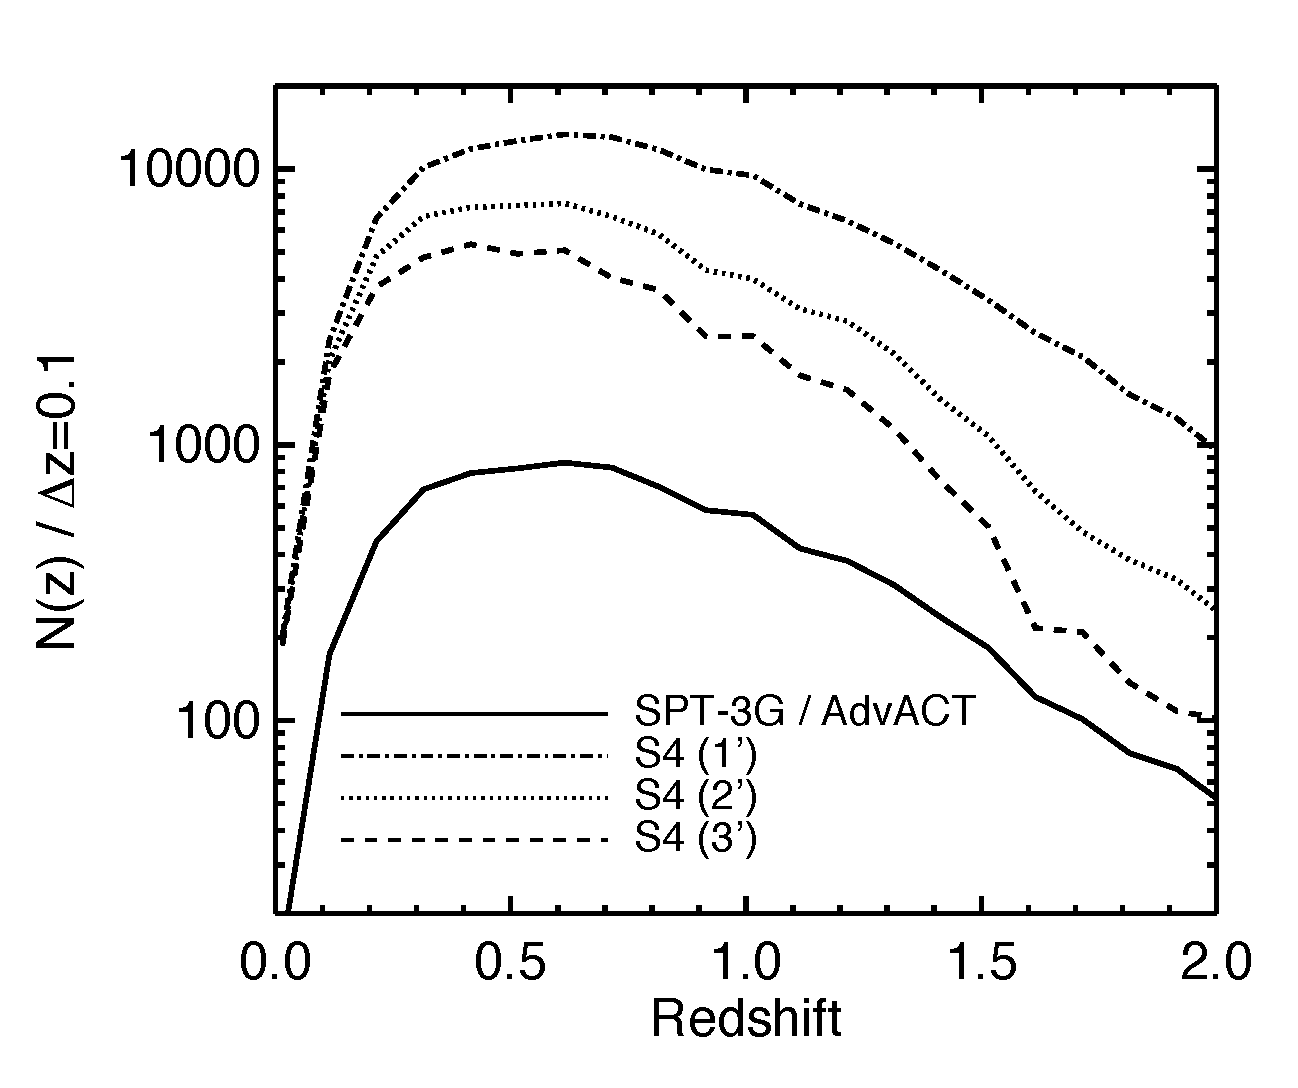
\includegraphics[width=0.49\textwidth]{DarkEnergy/dndz_s4.pdf}
\caption{(Left) The 50\% mass-completeness limits for three possible CMB-S4 instrumental configurations with either 1, 2, or 3 arc minute angular resolution.  For comparison, this can be compared with existing SZ-selected cluster catalogs from Planck \cite{Ade:2015mva}, SPT-SZ \cite{Bleem:2014iim}, and ACT \cite{Hasselfield:2013wf}, and future thresholds expected for the optical Dark Energy Survey and the X-ray eRosita survey \cite{Pillepich:2011zz}.  (Right) The projected cluster counts for the three possible CMB-S4 configurations described above.  For comparison, the projected cluster counts from the SPT-3G \cite{Benson:2014qhw} and AdvACT surveys.}
\label{fig:cluster_counts}
\end{center}
\end{figure} 

CMB-S4 will also enable a new means of calibrating cluster masses through CMB lensing.
Accurate masses are crucial for catalogs to provide constraints on dark energy and modified gravity.
With sufficient angular resolution, CMB-S4 opens tremendous possibilities for measuring cluster, more generally halo masses.    
  Figure \ref{fig:limits} shows an estimate of the mass sensitivity, expressed as the one-sigma mass uncertainty as a function of redshift, for two possible CMB-S4 configurations and compares them to planned CMB experiments. 


	The estimation is made assuming foreground subtraction to reach the quoted CMB map noise level at the given angular resolution.  The method (Melin \& Bartlett 2015) employs an optimal filter matched to the NFW profile and applied to reconstructions of the lensing potential with a quadratic estimator (Hu \& Okamoto 2002).  The method has already been successfully applied to the Planck cluster cosmology sample of more than 400 objects (Planck Collaboration XXIV 2015).  This figure shows the sensitivity obtained with just CMB temperature lensing reconstruction.  Including polarization will significantly improve it.  
	We see that the mass sensitivity remains flat with redshift, a remarkable property that enables mass estimation out to redshifts unreachable with galaxy shear measurements.  This is a powerful and unique capability of CMB lensing.  The figure also demonstrates the important gains attained with high angular resolution.  At one arcmin resolution, S4 achieves a mass sensitivity of $2 \times 10^{13}M_\odot$ with temperature alone.  This unprecedented sensitivity not only ensures robust mass estimation for cluster cosmology over the large redshift interval where S4 will detect clusters through the SZ effect, but also paves the way to numerous cluster and large-scale structure studies.  The rapidly increasing science reach enabled by high angular resolution, approaching one arcmin, is an important consideration in CMB-S4 objectives.  

\begin{figure}[t!]
\begin{center}
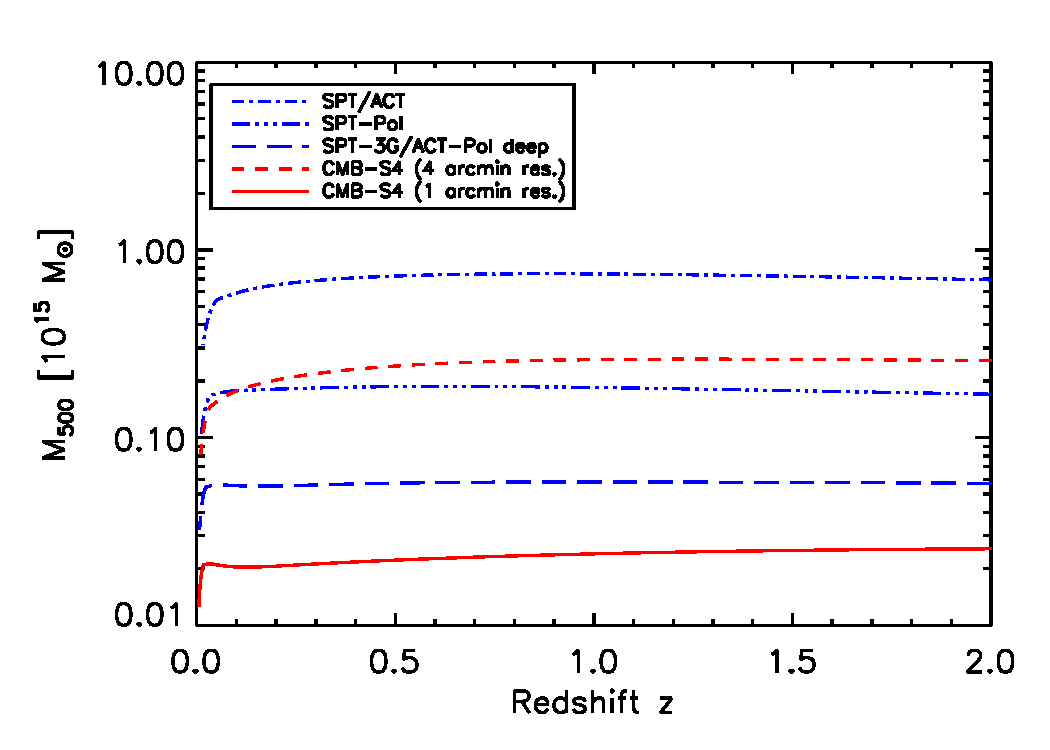
\includegraphics[width=0.65\textwidth]{DarkEnergy/m500lim_vs_z_1sigma_cmbs4_v1.pdf}
\caption{Cluster mass sensitivity of CMB lensing.}
\label{fig:limits}
\end{center}
\end{figure} 

\subsection{Lensing}

As described in the Lensing Chapter, the CMB lensing deflection map measures the projected mass density all the way back to the decoupling epoch at $z \sim 1100$, with the majority of the contributions coming from $z > 1$.  CMB lensing is also dominated by structure on large scales in the linear regime.  Thus,  CMB lensing provides a clean probe of a particular integral over the linear growth of structure,
e.g.~$\sigma_8(z)$,
weighted by distances. The lensing power spectrum shape is predicted from the background cosmology; shape deviations indicate scale-dependent effects on the growth, including those caused by modified gravity or the 
gravitational effects of dark energy.  CMB lensing complements other dark energy probes by providing
a handle on effects at high redshift, e.g. in so-called early dark energy scenarios.

Cross-correlating the CMB lensing with other tracers of structure further permits extraction of information about the growth rate of structure in the universe that is localized in redshift.  To the extent that other tracers have well-understood redshift distributions, cross-correlating a set of them to the CMB constitutes a tomographic study probing the evolution of the dark energy and its impact on the growth rate. The Lensing Chapter catalogs two broad categories of other tracers: galaxy density fields (and by extension the CIB) and galaxy shear maps. Combining lensing maps with maps of large scale flows from the kSZ will provide further constraints on the dark energy.

Another key contribution from CMB lensing to the study of dark energy will be its complementarity to other Stage IV experiments, including DESI and LSST, as well as EUCLID and WFIRST. (CMB Lensing chapter already mentions forecasting the improvement on calibrating multiplicative bias for LSST Ð would it make sense to move that here?) Not only will CMB lensing provide a new redshift kernel for tomography studies, it will also validate or improve the calibration for LSST, increasing its DE FOM by a factor of xxx.

%To include: forecasts for wa vs w0 (or whatever final parameterization is desired) for BOSS, then BOSS + CMB S4; for DESI+BOSS, then add in CMB S4; etc. 



\subsection{Kinematic SZ}

% Edited by F. de Bernardis
CMB-S4 will map with unprecedented precision the momentum field of the large scale structure via measurements of the kinematic Sunyaev Zel'dovich (kSZ) effect. Multi-frequency data can be used to remove other foregrounds and isolate the kSZ signal. CMB-S4 measurements with sufficient angular resolution can be used to reconstruct the diffuse kSZ anisotropy signal enabling sub-percent precision measurements of the amplitude of the matter density fluctuations $\sigma_8$ (see for example \cite{Calabrese:2014gwa}) while measurements of the patchy kSZ can place strong constraints on the time and duration of reionization.

The combination of CMB-S4 with data from galaxy surveys will be able to measure the kSZ effect associated with galaxy clusters, which is proportional to their peculiar momentum. The large scale structure momentum field is an important cosmological observable that can place strong constraints on the cosmological parameters \cite{Bhattacharya:2007sk,Kosowsky:2009nc,Mueller:2014nsa,Mueller:2014dba} complementary to density fluctuations field measurements. The mean pairwise velocity of galaxy clusters is sensitive to both the growth of structure and the expansion history of the universe and it is an excellent probe for gravity on large scales. Being a differential measurement it is also particularly stable against residual foregrounds that might survive the frequency cleaning process. In \cite{Mueller:2014nsa,Mueller:2014dba} it has been shown that a S4 survey with high resolution can constrain the redshift dependent growth of structure at $\lesssim 5\%$ precision in generic models allowing also for a redshift dependent equation of state of the dark energy. These measurements will be able to distinguish dark energy from modified gravity and will provide complementary constraints to redshift space distortions and weak lensing measurements, probing larger physical scales.

kSZ pairwise measurements can also constrain the sum of neutrino masses $M_{\nu}= \sum m_{\nu}$ with a $1\sigma$ uncertainty of $0.030$eV for a $1$ arcmin CMB-S4 overlapping 10000 deg$^2$ with a galaxy survey able to identify $M>10^{13}M_{\odot}$ clusters. With a 5 arcmin resolution separating the CMB background from the kSZ signal would be more difficult, providing  $\sigma_{M_{\nu}} = 0.076$eV (de Bernardis et al., in preparation). These forecasts include only priors on the 6 standard cosmological parameters from Planck temperatures data and show the potential of the kSZ pairwise signal to provide constraints on the neutrino mass. 

%
% Forecasts for the final book here or if more appropriate e.g. trigger type then embedded
% in the sections themselves

%
\section{Forecasts}
%

To forecast CMB-S4 performances on Dark Energy and Modified Gravity models we shall use the following specifications.
CMB-S4 is assumed to measure CMB fluctuations in temperature and polarization over $40 \%$ of the sky with a $1\,\mu {\rm K} \, {\rm arcmin}$ sensitivity in temperature and $1.4\,\mu {\rm K} \, {\rm arcmin}$ sensitivity in polarization, with a beam with $1\, {\rm arcmin}$ FWHM.
This is added to {\it Planck} measurements of CMB fluctuations on the remaining part of the sky with specifications from \cite{Adam:2015rua}. To reproduce the noise levels of real {\it Planck} measurements at large angular scales in polarization the E and B mode polarization sky fraction is reduced to $0.01$.
Along with CMB probes we shall use DESI to exploit the complementary sensitivity of LSS measurements and investigate the synergies with CMB-S4 in constraining DE/MG models.
We shall assume pessimistic specifications for the DESI survey as in \cite{Font-Ribera:2013rwa}.
When both CMB-S4 and DESI are considered we include in the forecast all the cross correlations between these two probes. \\
%
When a result is presented it is always marginalized over all the other parameters of the model. 
In particular, when considering DESI, we marginalize over a constant scale independent bias, different in all the survey redshift bins.
%

We use the the CosmicFish code \cite{Raveri:2016xof,Raveri:2016leq} to perform the forecast presented in this section. The CosmicFish code uses CAMB sources \cite{Lewis:1999bs,Challinor:2011bk} for all the $\Lambda$CDM cosmological predictions, uses EFTCAMB sources \cite{Hu:2013twa,Raveri:2014cka} for all models enclosed in the EFT framework and MGCAMB sources \cite{Zhao:2008bn,Hojjati:2011ix} for the Growth Index forecast.

\subsection{Trigger}

\begin{figure}[!tb]
\begin{center}
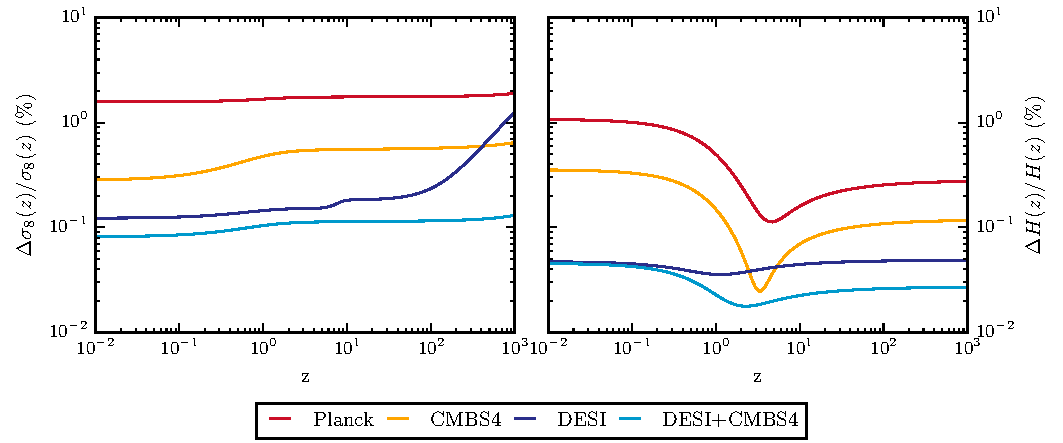
\includegraphics[width=1.0\textwidth]{DarkEnergy/1_Thomographic}
\caption{Relative $68\%$ C.L. error on $\sigma_{8}$ and $H$ as a function of redshift. Different colors correspond to different experiments, as shown in legend.}\label{fig:GrowthExpansion}
\end{center}
\end{figure}

We consider $\sigma_8(z)$, $H(z)$ and the growth index $\gamma_{L}$ as trigger parameters. Figure \ref{fig:GrowthExpansion} shows the relative error on $\sigma_8(z)$ and $H(z)$, assuming an underlying $\Lambda$CDM model. The central panel of Figure \ref{fig:MixedDEG} shows the marginal forecast constraint on $\gamma_{L}$. 

As we can see from the left panel of Figure \ref{fig:GrowthExpansion} CMB-S4 will improve on {\it Planck} determination of $\sigma_{8}(z)$ substantially, pushing the sensitivity to this parameter to sub-percent accuracy, especially at late times. 
This level of accuracy is comparable with DESI measurements that are, in turn, just a factor two tighter.
At early times CMB-S4 sensitivity to $\sigma_{8}$ is slightly lower but significantly better than DESI, as soon as redshift increases.
Noticeably when CMB-S4 and DESI are joined $\sigma_{8}$ gets constrained to $\sim 0.1\%$ at all times. The gain in the joint constraint is higher than the gain in sensitivity in going from CMB-S4 to DESI, thanks to the cross correlation between the two surveys.
%
A similar picture emerges from the right panel of Figure \ref{fig:GrowthExpansion} with the noticeable difference that CMB measurements have a peak in sensitivity around $z\sim 3$ that makes CMB-S4 stronger than DESI. The joint DESI CMB-S4 constraints reflect this. The addition of CMB-S4 measurements improves the constraint on the expansion history significantly at redshifts higher than three.

We considered $\sigma_8(z)$, $H(z)$ as trigger parameters because these levels of sensitivity will be the key to resolve tensions between different experiments. 
CMB measurements and LSS surveys display a marginal disagreement on the determination of the growth of cosmic structures but these tensions are still in a low statistical significance phase.
In particular {\it Planck} data are in tension with measurements of the Canada-France-Hawaii Telescope Lensing Survey (CFHTLenS) \cite{Joudaki:2016mvz} and the Kilo Degree Survey (KiDS) \cite{Hildebrandt:2016iqg} when considering the parameter $S_8\equiv \sigma_8\sqrt{\Omega_m/0.3}$. 
On the other hand the disagreement with the Dark Energy Survey (DES) is only marginal \cite{Abbott:2015swa}.
Two experiments with similar, high, sensitivity can either confirm or falsify these tensions to high statistical significance making CMB-S4 and DESI instrumental to each other.

In Table \ref{table:ForecastTensionS8} we investigate the expected statistical significance of these two tensions, when assuming the {\it Planck} mean $S_8$ value and the KiDS and DES ones. As we can see if we replace the {\it Planck} error with the forecasted CMB-S4 one the statistical significance of these tensions is limited by the sensitivity of the weak lensing surveys. When considering {\it Planck} and DESI sensitivities the statistical significance improves becoming almost decisive but still being limited by {\it Planck}. Only when considering both CMB-S4 and DESI we will achieve definitive sensitivity and this will allow us to establish whether these discrepancies are due to new physical phenomena or just statistical fluctuations.

\begin{table}[t!]
\begin{center}
\begin{tabular}{|c|c|c|c|} 
\hline
    				  Datasets 			& $\sigma_{S_8(z=0)}$  & Planck-KiDS tension & Planck-DES tension  \\
				  \hline
{\it Planck}  		& 		0.025	& - & -	\\
\hline
KiDS-450 		& 			0.038  	& $2.3 \, \sigma$ & -	\\
\hline
DES             &			0.06	 & - & $0.6 \, \sigma$	\\
\hline
CMB-S4       &			0.003  & 	$2.7 \, \sigma$ & $0.6 \, \sigma$	\\
\hline
{\it Planck} and DESI            &   0.0009	& 	$4.1 \, \sigma$ & $1.5 \, \sigma$	 \\
\hline
CMB-S4 and DESI  &   0.0004	 & 	$33 \, \sigma$ & $12 \, \sigma$			\\
\hline
\end{tabular}
\caption{Forecasted constraints on $S_8\equiv \sigma_8\sqrt{\Omega_m/0.3}$ and statistical significance of the discrepancy between {\it Planck} and the DES and KiDS surveys.}
\label{table:ForecastTensionS8}
\end{center}
\end{table}

The power of CMB-S4 in constraining the growth of structures and its synergy with LSS surveys clearly shows when considering the Growth Index $\gamma_{L}$. As we can be see from both the central panel of Figure \ref{fig:MixedDEG} and Table \ref{table:ForecastGammaConstEFT} CMB-S4 will give stronger constraints with respect to {\it Planck} due to the additional leverage of CMB lensing. These constraints will be comparable with DESI ones and displaying a slightly different degeneracy with the amplitude of scalar perturbations.
Leveraging on the precision of both CMB and LSS measurements, the joint constraints with CMB-S4 and DESI are significantly stronger than the single probes considered alone.

\subsection{Equation of motion parametrization}

\begin{table}[t!]
\begin{center}
\begin{tabular}{|c|c|c|c|} 
\hline
Datasets 			&  $r$ fiducial & $\sigma ( r )$  & $\sigma ( c_{\rm GW}^2 )$ \\
\hline
\hline
CMB-S4               & 0.05 & 0.002 & 0.05 \\
\hline
CMB-S4               & 0.01 & 0.001 & 0.1 \\
\hline
CMB-S4               & 0.001 & 0.0008 & - \\
\hline
CMB-S4 + DESI     & 0.001 & 0.0007 & - \\
\hline
\end{tabular}
\caption{Forecast $68\%$ C.L. marginal constraints on the tensor to scalar ratio ($r$) and the speed of gravitational waves for different fiducial values of $r$.}
\label{table:ForecastCT}
\end{center}
\end{table}

We describe deviations of the speed of GWs from the speed of light, with the parameter $c^2_{\rm GW}$. If the effect of primordial GWs on the B-mode polarization of the CMB is detected then the same observations will be capable of constraining their propagation speed at the time of recombination.
In the left panel of Figure \ref{fig:MixedDEG} we show the marginalized joint forecast constraint on the tensor to scalar ratio and the speed of GWs for a fiducial value of $r=0.01$ and $c_{\rm GW}^2=1$. In Table \ref{table:ForecastCT} we show the expected marginal constraints when changing the fiducial value of $r$.

As we can see, if $r$ is detected in the $0.05$ range, CMB-S4 measurements will provide a $5\%$ bound on the speed of GWs at the time of recombination.
As soon as the GW induced component in the B-mode polarization spectrum, becomes weak the bound on the GW's speed gets looser. If the fiducial is $r=0.01$ then CMB-S4 measurements will provide a $10\%$ bound. If $r=0.001$ then the statistical significance of the tensor induced B-mode component detection weakens and correspondingly the speed of GWs gets unconstrained.

When $r=0.01$ we also notice a slight degeneracy between the speed of GWs at recombination and the tensor to scalar ratio. Correspondingly CMB-S4 measurements will be more sensitive to the sum of these two parameters. This degeneracy is alleviated as soon as the fiducial $r$ value is increased and becomes negligible for $r=0.05$.

We stress here that all the other experiment combinations considered in this section could not constrain the speed of GWs thus CMB-S4 will give us the unique opportunity to measure this quantity at the time of recombination.

\subsection{Theory parametrization}

\begin{table}[t!]
\begin{center}
\begin{tabular}{|c||c||c|c|c||c|c|c|} 
\hline
Datasets 			& $\sigma ( \gamma_{\rm L} )$  & $\sigma ( \Omega_0 )$ & $\sigma ( \gamma_0^{(2)} )$ & $\sigma ( \gamma_0^{(3)} ) $ & $\tilde{M}_0$ & $\alpha_0^{\rm B}$ & $\alpha_0^{\rm T}$    \\
\hline
\hline
{\it Planck}  		& 0.02 & 0.03 & 0.4 & 0.01 & 0.03 & 0.02 & 0.02 \\
\hline
CMB-S4       & 0.007 & 0.02 & 0.1 & 0.01 & 0.02 & 0.02 & 0.008 \\
\hline
DESI            & 0.007 & 0.2 & 0.4 & 0.1 & 0.02 & 0.07 & 0.03 \\
\hline
CMB-S4 + DESI  & 0.003 & 0.01 & 0.05 & 0.003 & 0.006 & 0.02 & 0.001 \\
\hline
\end{tabular}
\caption{Forecast $68\%$ C.L. marginal constraints on different models: the trigger parameter $\gamma_{\rm L}$; constant EFT couplings $\Omega_0$, $\gamma_0^{(2)}$ and $\gamma_0^{(3)}$; constant Horndeski couplings $\tilde{M}_0$, $\alpha_{\rm B}$ and $\alpha_{\rm T}$.}
\label{table:ForecastGammaConstEFT}
\end{center}
\end{table}

\begin{table}[t!]
\begin{center}
\begin{tabular}{|c||c|c||c|c|c|c|c|c|} 
\hline
Datasets 			& $\Omega_{\rm early}$ & $\Omega_{\rm late}$ & $\tilde{M}_{\rm early}$ &  $\tilde{M}_{\rm late}$ & $\alpha^{\rm B}_{\rm early}$ & $\alpha^{\rm B}_{\rm late}$ & $\alpha^{\rm T}_{\rm early}$  & $\alpha^{\rm T}_{\rm late}$   \\
\hline
\hline
{\it Planck}  		& 0.08 & 0.05 & 0.2 &  0.1 & 0.05 & 0.2 & 0.03 & 0.04 \\
\hline
CMB-S4       &  0.04 &  0.04 & 0.05 & 0.02 & 0.05 & 0.1 & 0.02 & 0.01 \\
\hline
DESI            & 0.3 & 0.2 & 1.0 & 0.04 & 0.4 & 0.4 & 0.08 & 0.03 \\
\hline
CMB-S4 + DESI  &  0.03 &  0.02 & 0.04 & 0.007 & 0.04 & 0.08 & 0.02 & 0.002\\
\hline
\end{tabular}
\caption{Forecast $68\%$ C.L. marginal constraints on early and late time values of different EFT couplings.}
\label{table:ForecastAlphaAtan}
\end{center}
\end{table}

We consider two parametrization basis for the functions describing the EFT of cosmic acceleration and, for the sake of simplicity, we focus on the Horndeski class of models \cite{Horndeski:1974wa}.
%
The first parametrization is obtained by making the couplings in action (\ref{Eq:EFTaction}) dimensionless, as in \cite{Hu:2014oga}.
The second one consists in re-parametrizing the couplings explicitly targeting the phenomenological features of Horndeski, as in \cite{Bellini:2014fua}.
%
In both cases we consider two functional forms: we assume all the couplings constant in time; we allow all the EFT couplings to have different early and late time values, with a smooth transition in between, inspired by \cite{Linder:2015rcz}. Specifically this second parametrization is given by $f(a)= 1/2 (f_{\rm early} + f_{\rm late}) + ( f_{\rm late} -f_{\rm early} ) {\rm ArcTan}[(a - a_T)/\Delta a]/\pi$ where $f_{\rm early}$ and $f_{\rm late}$ are respectively the early and late time values of the considered EFT function, $a_T$ is the transition scale factor assumed to correspond to $z=10$ and $\Delta a=0.01$ is the transition sharpness. 
%

In Figure \ref{fig:ConstantEFT} and Table \ref{table:ForecastGammaConstEFT} we show the forecast constraints on constant EFT couplings. As we can see the sensitivity of CMB probes are unmatched when measuring the conformal coupling to gravity $\Omega_0$. 
CMB-S4 measurements, in addition, are found to be the most constraining measurements on the other two EFT higher order operators, $\gamma_0^{(2)}$ and $\gamma_0^{(3)}$. Confirming the picture previously presented, the synergy between CMB-S4 measurements and DESI, results in much tighter constraints on all the considered parameters.
For all the probes considered the kinetic operator, $\gamma_0^{(1)}$, is found to be unconstrained. 

A similar picture also emerges from the forecast constraints on Horndeski couplings, with CMB-S4 providing the tightest bounds, as we can see from Figure \ref{fig:ConstantAlpha} and Table \ref{table:ForecastGammaConstEFT}. 
When considering the effective Planck mass $\tilde{M}_0$ and the tensor speed excess, $\alpha_0^{\rm T}$, DESI and {\it Planck} sensitivities are comparable while CMB-S4 is a factor 1.5 and 2.5 stronger, respectively. 
CMB measurements, on the other hand, are the most powerful at constraining the braiding coefficient $\alpha_0^{\rm B}$ and we can notice that {\it Planck} measurements are slightly stronger than CMB-S4 ones leveraging on the constraining power of large angular scales. 
As expected, combining CMB-S4 to DESI, results in a significant improvement with respect to the single probes alone.
As in the constant EFT case the scalar field kineticity $\alpha_0^{\rm K}$ is unconstrained.

When considering all the EFT couplings having different values at early and late times we found that early times changes are constrained by physical viability requirements and late time values have comparable bounds with respect to the constant case considered before.
The only EFT coupling that does not display this behavior is the conformal one, $\Omega(a)$, and the corresponding forecast constraints are shown in the right panel of Figure \ref{fig:MixedDEG} and Table \ref{table:ForecastAlphaAtan}. For these parameters we find that marginalization slightly degrades the forecast bounds with respect to the constant case. Moreover we find that data are more sensitive to the sum of these two parameters rather than their difference. When CMB-S4 is combined to DESI this degeneracy in parameter space is relieved.

Horndeski couplings in turn display a qualitatively different picture, as we can see from Figure \ref{fig:VariationAlpha} and Table \ref{table:ForecastAlphaAtan}.
Not surprisingly CMB measurements are generally stronger than LSS surveys at constraining the early time values of these functions, i.e. $\tilde{M}_{\rm early}$, $\alpha^{\rm T}_{\rm early}$ and $\alpha^{\rm B}_{\rm early}$. However CMB-S4 measurements, leveraging on both the early and late time constraining power of CMB and CMB lensing, are sensitive to both early and late time values, to unmatched accuracy.


\begin{figure}[!tb]
\begin{center}
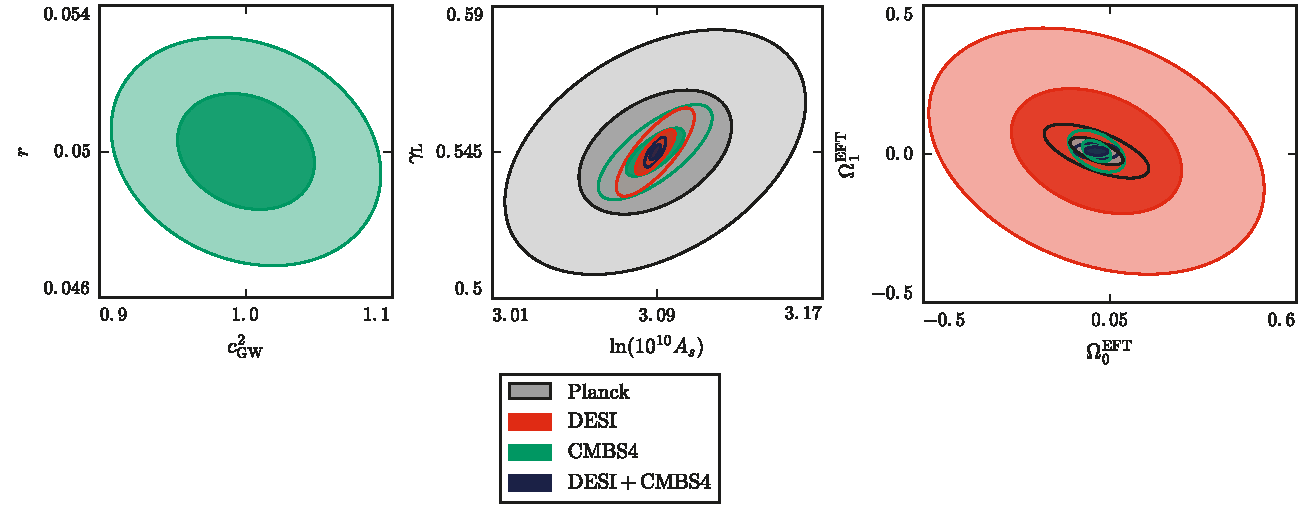
\includegraphics[width=1.0\textwidth]{DarkEnergy/2_mixed}
\caption{Forecast marginalized constraints on different models. The left panel shows the joint constraints on the tensor to scalar ratio and the speed of gravitational waves. The central panel shows the joint constraints on the growth index and the amplitude of scalar perturbations. The right panel shows the joint constraints on relative variations of the gravitational constant at early times $\Omega_0^{\rm EFT}$ and late times $\Omega_1^{\rm EFT}$. Different colors correspond to different experiments, as shown in legend. The darker and lighter shades correspond respectively to the 68\% C.L. and the 95\% C.L. regions.}\label{fig:MixedDEG}
\end{center}
\end{figure}

\begin{figure}[!tb]
\begin{center}
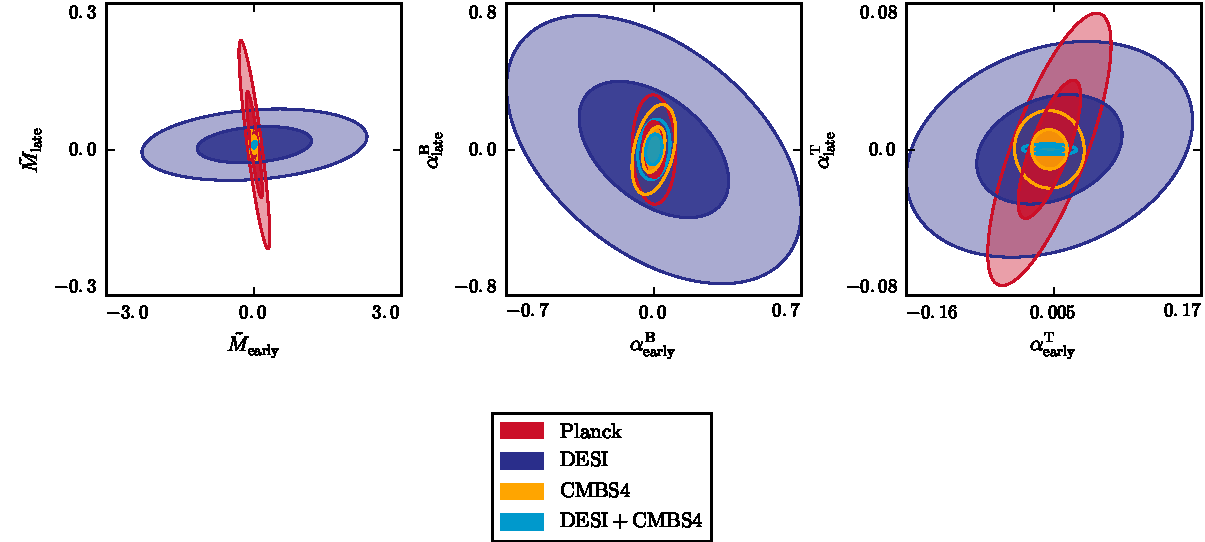
\includegraphics[width=1.0\textwidth]{DarkEnergy/11_alpha_atan}
\caption{Forecast marginalized constraints on Horndeski couplings. The left panel shows the joint constraints on the effective Planck mass at early times $\tilde{M}_{\rm early}$ and late times $\tilde{M}_{\rm late}$. The central panel shows the joint constraints on the Horndeski braiding coefficient at early times $\alpha^{B}_{\rm early}$ and late times  $\alpha^{B}_{\rm late}$. The right panel shows the joint constraints on the Horndeski tensor speed excess coefficient at early times $\alpha^{T}_{\rm early}$ and late times  $\alpha^{T}_{\rm late}$. The Horndeski kineticity coefficient is unconstrained by all the experimental combinations considered. Different colors correspond to different experiments, as shown in legend. The darker and lighter shades correspond respectively to the 68\% C.L. and the 95\% C.L. regions.}\label{fig:VariationAlpha}
\end{center}
\end{figure}

\begin{figure}[!tb]
\begin{center}
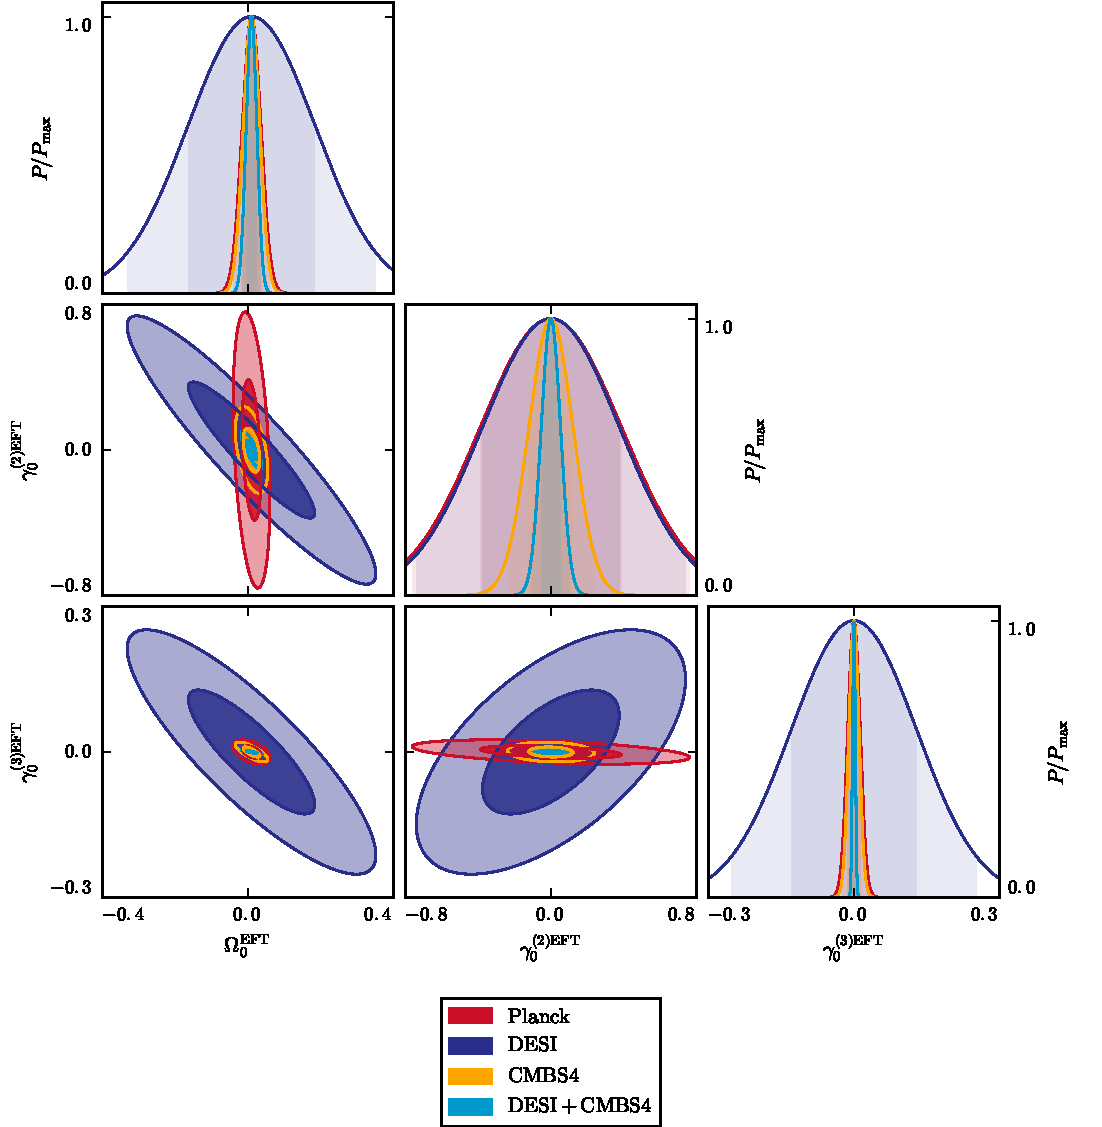
\includegraphics[width=1.0\textwidth]{DarkEnergy/6_ConstEFT}
\caption{Forecast marginalized constraints on constant EFT couplings: $\Omega_0^{\rm EFT}$, $\gamma_{0}^{(2){\rm EFT}}$ and $\gamma_{0}^{(3){\rm EFT}}$. Different colors correspond to different experiments, as shown in legend. The darker and lighter shades correspond respectively to the 68\% C.L. and the 95\% C.L. regions.}\label{fig:ConstantEFT}
\end{center}
\end{figure}

\begin{figure}[!tb]
\begin{center}
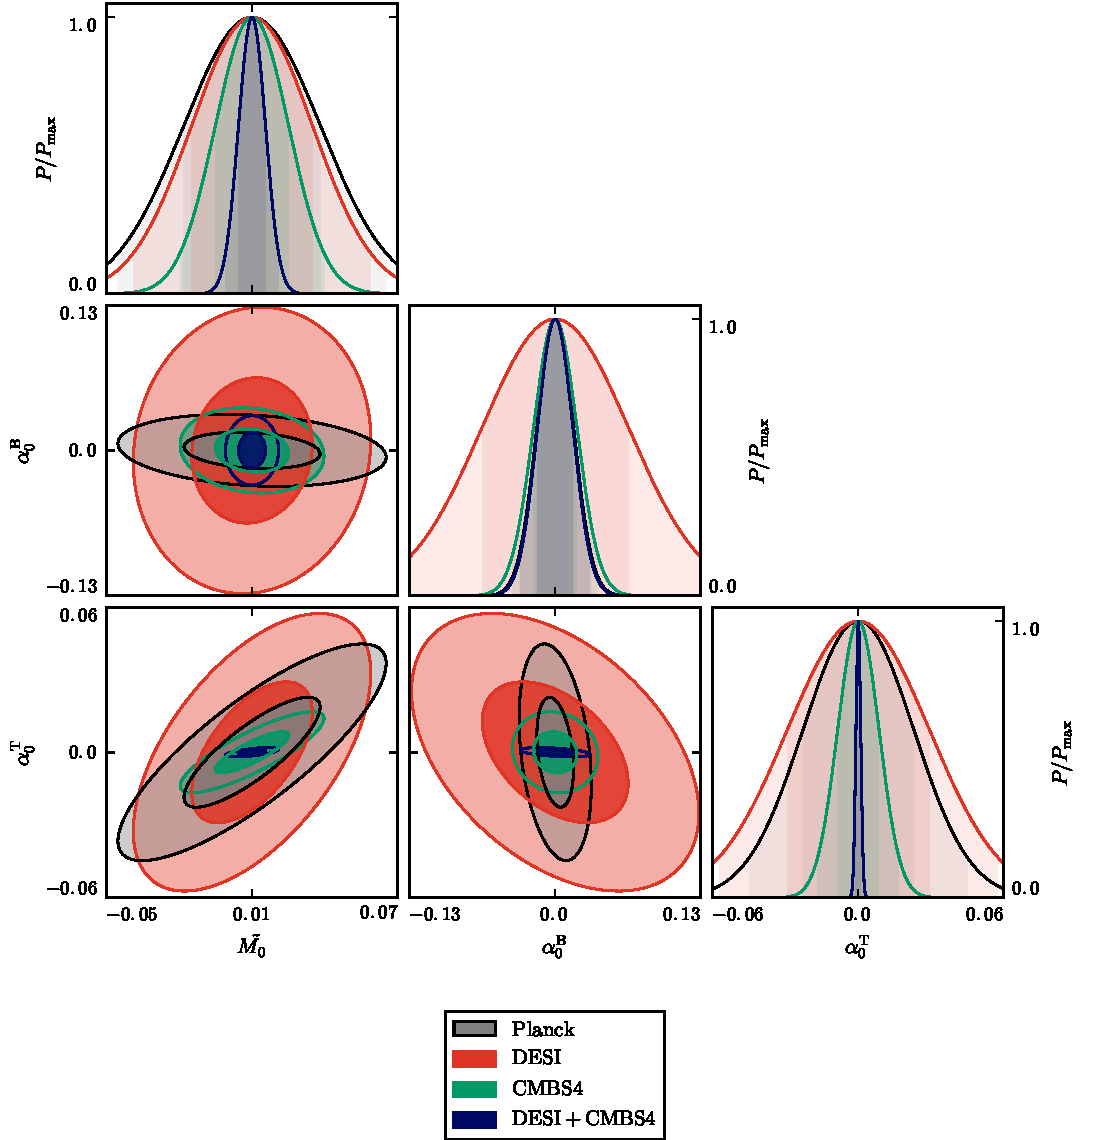
\includegraphics[width=1.0\textwidth]{DarkEnergy/7_Const_alpha}
\caption{Forecasted marginalized constraints on constant Horndeski couplings: $\tilde{M}_{0}$, $\alpha^{\rm B}_0$ and $\alpha_0^{\rm T}$. Different colors correspond to different experiments, as shown in legend. The darker and lighter shades correspond respectively to the 68\% C.L. and the 95\% C.L. regions.}\label{fig:ConstantAlpha}
\end{center}
\end{figure}

\section{Summary}
Dark Energy is an elusive cosmological component which drives many current efforts in cosmology. The model parameter space is broad, and CMB-S4 provides a powerful probe to distinguish different models of dark energy through their effects on both the CMB power spectrum itself and the lensing of the CMB, bringing us closer to the goal of understanding and ruling out competing models of this strange compenent in our cosmological model.
%\bibliography{cmbs4}

%%
%% Populate the .bib file with entries from SPIRES Bibtex (preferred)
%% or ADS Bibtex (if no SPIRES entry).
%%  SPIRES will also supply the CITATION line information; please include it.
%%


